\section{Introduction}
\label{sec:intro}
\subsection{Motivation}
Galaxies have morphology that can be split into two main categories: spiral and elliptical. 
The differences between them are fairly obvious from images: spiral galaxies are disk shaped and have curved arms extending out from the centre, while elliptical galaxies are shaped like an three dimensional blob that is brighter in the middle. 

\begin{figure}[h]
	\centering
	\captionsetup{justification=centering,width=.8\linewidth}
	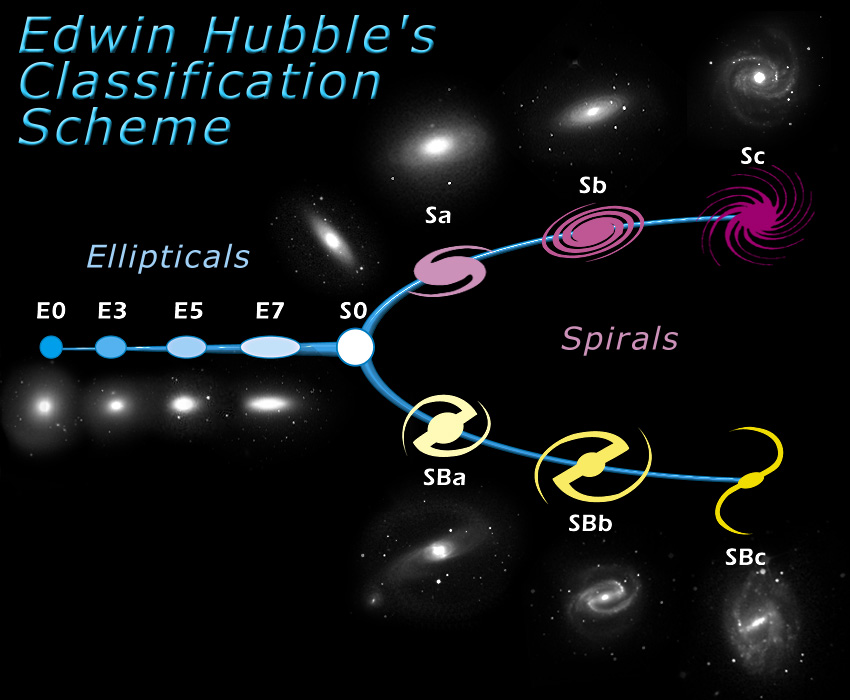
\includegraphics[scale=0.7]{Figures/TuningFork.jpg}
	\caption{Edwin Hubble's 'Tuning Fork' classification scheme. Galaxies are classified into two main categories, spiral and elliptical, with further sub-classifications representing minute changes \cite{TuningFork}.}
	\label{fig:tuningfork}
\end{figure}


There are many more differences between the two galaxy morphologies that are not as glaringly.  
For example, Spiral galaxies tend to be bluer than their elliptical cousins. 
Dense spiral arms are the birthplace of new stars, which excite gas around them and cause it to glow a blue colour. 
Elliptical galaxies lack the gas and dust required to form new stars, and therefore tend to be redder. 
When two galaxies of any type collide, they eventually form a large elliptical galaxy. 
Elliptical galaxies are much more common near the centre of galaxy clusters for this reason, and can be many times larger than their spiral counterparts.
Classifying galaxies based on their morphology therefore has a large impact on research in many fields of astronomy, including things from galactic dynamics to the age of the Universe!

Humans can easily distinguish between the two forms given the collected data is high enough resolution. 
There is one major problem in this field of research that is rather unexpected - we have too much data available to look through and separate! 
The Sloan Digital Sky Survey is one of the newer collection surveys that is starting to monopolize the field. SDSS has a list of over 200,000,000 individual galaxies across more than one third of the night sky\cite{SDSS}!

\subsection{Approach}
This is where data science comes in - a neural network trained to classify images into these categories would be extremely useful to many astronomers. 
A convolutional neural network (CNN) should be able to identify galaxies much faster than humans, with comparable accuracy.












